\documentclass[a4paper,12pt]{article}
\usepackage{../packages/coursCollege}
\newcommand{\Chapitre}{Algèbre}
\renewcommand{\path}{../}

\usepackage[    %backend=biber, 
    natbib=true,
    style=numeric,
    sorting=none]{biblatex}  % Load biblatex for bibliography handling
\addbibresource{biblio-der.bib}  
\renewcommand\refname{Sources}
\renewcommand{\cours}{1MA~--~EG~--~ns~--~2025-2026}
\begin{document}
\tocloftpagestyle{fancy}
% Reduce space between section entries
\setlength{\cftbeforesecskip}{2pt}

% Reduce indentation for section entries
\setlength{\cftsecindent}{1em}

\begin{center}
	{\bfseries \Huge Algèbre}

	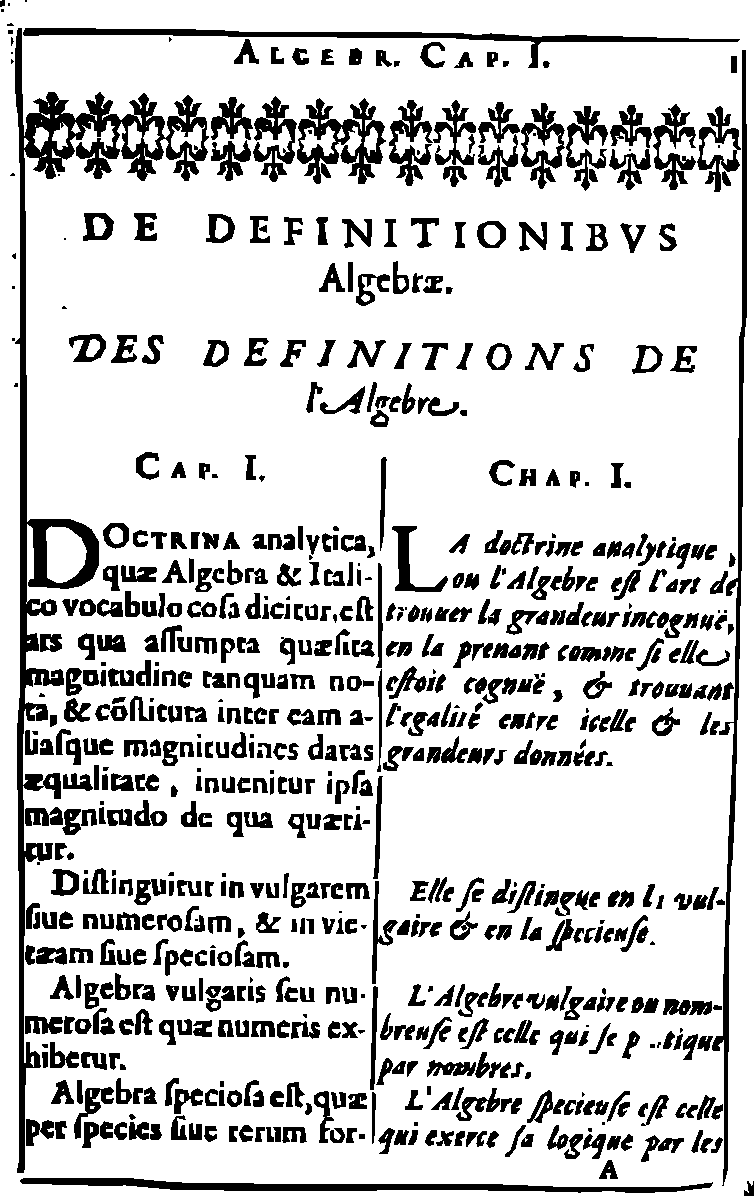
\includegraphics[scale=0.6]{../medias/1M/fiches/algebreFront}


Hérigone, Pierre. Cours mathématique. Vol. 1. Paris, 1634, p. A1.
\end{center}

\vspace{-1cm}

\tableofcontents

\newpage
\section{Calcul littéral}

\subsection{Techniques de factorisation}

 Pour factoriser il faut 
  \begin{enumerate}
	  \item mettre en évidence le plus grand facteur possible;
	  \item vérifier si on se trouve face à une identité remaquable;
	  \item appliquer la technique des groupements pour révéler une factorisation plus poussée;
	\item réduire les expressions obtenues;
	\item recommencer les étapes ci-dessus.
\end{enumerate}
Factoriser une expression est un problème difficile, il n'y a pas de marche à suivre précise, mais il faut maîtriser les techniques suivantes afin reconnaître les situations dans lesquelles il est nécessaire de les appliquer.
\begin{description}
\item[Mise en évidence] On détermine le pgcd des coefficients et la partie littérale commune de chacun des termes.
\item[Identités remarquables] On applique les schémas vus dans la théorie pour nous aider à choisir de quelle identité il s'agit.
\item[Technique des groupements] On essaye de faire apparaître un facteur commun à plusieurs termes, mais pas à tous en même temps.
\end{description}

\begin{exemple}
	Exemple de factorisation avec groupements
	\tcblower
\vspace{5cm}

\end{exemple}
Les groupements peuvent être égaux au signe près. On multiplie par $1=(-1)^2$ pour obtenir un changement de signe du groupement.
%\[(x-y)(3x-4)=(-1)^2(x-y)(3x-4)=(-1)(x-y)(-1)(3x-4)=(y-x)(4-3x)\]
\begin{exemple}
	Retrouver un groupement au signe près
	\tcblower
\vspace{6cm}

\end{exemple}
Les techniques s'enchaînent. Voici quelques exemples.

\begin{exemple}Identité remarquable avec groupements
	\tcblower
	\vspace{6cm}	

\end{exemple}

\begin{exemple}
	 Identité remarquable pour faire apparaître un groupement
	\tcblower
	\vspace{8cm}	

\end{exemple}

\begin{exemple}
	Groupement pour faire apparaître une identité
	\tcblower
	\vspace{7cm}	

\end{exemple}

\begin{exercice}
	\tcblower
Factoriser le plus possible les expressions suivantes.
  \begin{tasks}(2)
  	\task $(7x-1)^2-(5x+2)^2$
	\task $(4x-1)^2-9(3-x)^2$
	\task* $2x^2-4x+2-3(x-1)(2x+1)$
	\task* $25x^2+(5x-3)(2x+7)-9+(6-10x)(x-3)$
  \end{tasks}
\end{exercice}

\section{Équations du premier degré}
\subsection{Généralités}
\begin{definition}
	équation
	\tcblower
	Une {\bfseries équation} est une expression mathématique avec un membre de gauche, un signe égalité et un membre de droite. Les membres de gauche et de droite sont des expressions littérales contenant des inconnues.
	\begin{center}
\begin{tikzpicture}[
    box/.style={draw, minimum width=2cm, minimum height=1cm},
    mylabel/.style={font=\small\itshape}
]
    % Left box (LHS)
    \node[box] (lhs) at (0,0) {$\ldots$};
    
    % Equal sign
    \node[font=\Large] (eq) at (3,0) {$=$};
    
    % Right box (RHS)
    \node[box] (rhs) at (6,0) {$\ldots$};
    
    % Arrows and labels
    \draw[Latex-] (lhs.north) -- ++(0,0.5) node[above, mylabel] {membre de gauche (mdg)};
    \draw[Latex-] (eq.north) -- ++(0,0.5) node[above, mylabel] {\text{signe égal}};
    \draw[Latex-] (rhs.north) -- ++(0,0.5) node[above, mylabel] {membre de droite (mdd)};
\end{tikzpicture}
\end{center}
\end{definition}
\begin{definition}
	degré
	\tcblower
	Le {\bfseries degré} d'une équation est le plus haut degré d'un monôme apparaissant dans l'équation.
\end{definition}
\begin{definition}
	solution d'une équation
	\tcblower
	Une {\bfseries solution d'une équation} est un nombre ou un tuple de nombres qui satisfait l'égalité lorsqu'on substitue à la place de l'inconnue ou des inconnues.
\end{definition}
\begin{exemple}
	Solution d'une équation
	\tcblower
\vspace{6cm}

\end{exemple}
On note avec un ensemble l'ensemble de toutes les solution d'une équation $S=\{\ldots\}$ 
\begin{definition}
	équations équivalentes
	\tcblower
	Deux équations sont appelées {\bfseries équivalentes} si elles ont le même ensemble de solutions. 
\end{definition}
\begin{exemple}
	Équations équivalentes
	\tcblower
\vspace{5cm}

\end{exemple}
Résoudre une équation c'est déterminer une équation équivalente dans laquelle la solution peut être lue facilement. Par exemple, l'équation $2x+3=4x-1$ est équivalente à l'équation $x=2$. La deuxième équation permet de déduire la solution. Deux principes permettent de passer d'une équation à une équation équivalente.
\begin{exemple}
	Principe d'équivalence 1 [PE1]
	\tcblower
\vspace{8cm}

\end{exemple}
\begin{exemple}
	Principe d'équivalence 2 [PE2]
	\tcblower
\vspace{8cm}

\end{exemple}
\newpage
\subsection{Équations du premier degré}

Une équation du premier degré à une inconnue est de la forme $ax+b=cx+d$ avec $a,b,c,d\in \R$.
\begin{exemple}
	Résolution d'une équation du premier degré
	\tcblower
\vspace{7cm}

\end{exemple}
Ce type d'équation peut avoir une unique solution, aucune solution ou une infinité de solutions~:
\begin{itemize}
	\item[] si $a\neq c$ alors l'équation admet une unique solution;
	\item[] si $a=c$ est $b\neq d$ alors $S=\emptyset$;
	\item[] si $a=c$ et $b=d$ alors $S=\R$.
\end{itemize}
\begin{exemple}
	Les trois types d'ensemble de solutions
	\tcblower
\vspace{10cm}

\end{exemple}
\newpage
On résout, comme exemple, quelques équations.
\begin{exemple}
	Équation avec des fractions
	\tcblower
\vspace{10cm}

\end{exemple}
\begin{exemple}
	Équation avec de la distributivité
	\tcblower
\vspace{10cm}

\end{exemple}
\newpage
\subsection{Équation contenant un paramètre}
\begin{exemple}
	Une première équation avec un paramètre (discussion)
	\tcblower
	\vspace{8cm}

\end{exemple}


\begin{exemple}
	Reconnaître une équation avec un paramètre
	\tcblower
	\vspace{6cm}

\end{exemple}

\begin{exemple}
	Exemple 1 $(k+2)x=8$
	\tcblower
	\vspace{6cm}

\end{exemple}


\begin{exemple}
	Exemple 2 $a(x-3)=5a$
	\tcblower
	\vspace{6cm}

\end{exemple}

\begin{exemple}
	Exemple 3 $(p-1)x+3=3x$ 
	\tcblower
	\vspace{6cm}

\end{exemple}

\begin{exemple}
	Exemple 4 $(m+3)x+7=mx+10$
	\tcblower
	\vspace{6cm}

\end{exemple}
\begin{exercice}
	\tcblower
Résoudre dans $\R$ pour $x$.
\begin{tasks}(2)
	\task $4 m x-8-11 m=3+2 m$
	\task $5x-3p=2x-7$
	\task $9r^2x+2r=4x-5$
\end{tasks}
\end{exercice}

\newpage
\subsection{Résolution d'un problème du premier degré}
Les équations sont l'outil principal de résolution de problème en mathématiques. 

Voici les étapes à suivre pour résoudre un problème à l'aide d'une équation.

{\bfseries Partie 1\,: Déterminer l'équation}
\begin{enumerate}[1)]
	\item Lire le problème autant de fois que nécessaire pour bien comprendre et interpréter la situation.

		{\bfseries Faire un schéma si besoin};
	\item déterminer les deux quantités à comparer, elles deviendront les deux membres de l'équation;
	\item poser une inconnue qui permet d'exprimer les quantités à égaliser;
	\item écrire les deux membres de l'équation en fonction de l'inconnue. L'inconnue devrait apparaître dans au moins un des deux membres.
\end{enumerate}
{\bfseries Partie 2\,: Résoudre l'équation}
\begin{enumerate}[1),resume]
	\item Résoudre l'équation avec les principes d'équivalence.
\end{enumerate}
{\bfseries Partie 3\,: Interpréter le résultat et conclure}
\begin{enumerate}[1),resume]
	\item Vérifier la cohérence du résultat avec le choix de l'inconnue;
	\item Interpréter la valeur obtenue et répondre à la question posée dans l'énoncé.
\end{enumerate}
\begin{exemple}
	\tcblower
	[Exemple 1]
	
\vspace{6.5cm}

\end{exemple}
\begin{exemple}
	\tcblower
	
\vspace{6.5cm}

\end{exemple}
\newpage

Déterminer la mesure du côté du carré afin que les périmètres du carré et du triangle soient égaux.
\begin{center}
	\begin{tikzpicture}[scale=0.8]
    % Define the length of the side of the square and triangle
    \def\side{4}

    % Define points for the square
    \tkzDefPoint(0,0){A} % bottom-left of the square
    \tkzDefPoint(9,0){F}
    \tkzDefPoint(\side,0){B} % bottom-right of the square
    \tkzDefSquare(A,B) \tkzGetPoints{C}{D} % Top points of the square

    % Draw the square
    \tkzDrawPolygon(A,B,C,D)

    % Right angle marks for the square
    \tkzMarkRightAngle[size=0.3](A,B,C)
    \tkzMarkRightAngle[size=0.3](B,C,D)
    \tkzMarkRightAngle[size=0.3](C,D,A)
    \tkzMarkRightAngle[size=0.3](D,A,B)

    % Define points for the equilateral triangle starting from point B
    \tkzDefEquilateral(B,F) \tkzGetPoint{E} % E is the third point of the triangle
    \tkzDrawPolygon(B,F,E) % Draw the equilateral triangle

    % Mark equal sides of the triangle
    \tkzMarkSegments[mark=|](B,F B,E F,E)
    \tkzMarkSegments[mark=||](A,B B,C C,D D,A)

    % Draw the dimension line from A to E and label it 20 cm
    %\tkzDrawSegment[<->,blue](A,E)
    %\node[below] at ($(A)!0.5!(E)$) {20 cm};

\end{tikzpicture}
\end{center}

\begin{exemple}
	\tcblower
	
\vspace{20cm}

\end{exemple}
\section{Équations du second degré}
\subsection{Théorème du produit nul}

\begin{exemple}
	Théorème du produit nul
	\tcblower
	\vspace{10cm}	

\end{exemple}

Grâce à la factorisation et au théorème du produit nul, on peut résoudre une équation de dégré supérieur en résolvant plusieurs équations de dégré inférieur.

\begin{exemple}
	Résoudre $x^3(x+2)^2=x^2(x+2)^2$
	\tcblower
	\vspace{10cm}

\end{exemple}

\begin{exemple}
	Résoudre $x^2+2x-1=0$
	\tcblower
	En appliquant les étapes suivantes\,:

	\begin{tasks}
\task $\left[P E_1\right]:$ +2
\vspace{1.5cm}
\task factoriser le membre de gauche
\vspace{1.5cm}
\task $\left[P E_1\right]:$ $-2$
\vspace{1.5cm}
\task factoriser le membre de gauche
\vspace{1.5cm}
\task $\left[P N\right]$
\vspace{1.5cm}
	\end{tasks}
\end{exemple}

\begin{exemple}
	Résoudre $(8x+1)^2-(2x-3)^2=0$
	\tcblower
	\vspace{11cm}	
\end{exemple}
\newpage
\subsection{Complétion du carré}
La complétion du carré est une technique qui permet de résoudre une équation du second en se ramenant aux techniques de factorisation connues.
\begin{exemple}
	$x^2-8x+4=0$
	\tcblower
	\vspace{10cm}	

\end{exemple}

\begin{exemple}
	$2x^2+3x-2=0$
	\tcblower
	\vspace{10cm}	

\end{exemple}
\newpage
Voici les étapes à suivre pour l'appliquer sur l'équation générale 
\[ax^2+bx+c=0.\]
	\vspace{20cm}

En suivant ces étapes, on remarque que l'on vient de démontrer la formule de résolution d'équation du second degré. On appellera cette formule dans le cours la \emph{formule du deuxième degré}.
Résoudre les équations suivantes à l'aide de la méthode de complétion du carré.
\begin{tasks}(2)
 \task $3 x^2+24 x+48=0$
 \task $6 x^2+7 x-20=0$
 \task $2 x^2-6 x+2=0$
 \task $-x^2+4 x-2=0$
\end{tasks}

\subsection{Utilisation de la formule du deuxième degré}
On a démontré la formule suivante pour résoudre une équation du second degré.

	\vspace{12cm}

\begin{exemple}
	$2x^2-x+3=0$
	\tcblower
	\vspace{10cm}
\end{exemple}
\begin{exemple}
	$2x^2-x-6=0$
	\tcblower
	\vspace{10cm}
\end{exemple}
\begin{exemple}
	$2x^2-x+3=3x^2+x+2$
	\tcblower
	\vspace{10cm}
\end{exemple}

Résoudre les équations dans $\mathbb{R}$, à l'aide de la formule du deuxième degré~:
\begin{tasks}
\task $3 x^2-4 x-2=0$
\task $6-3 x+x^2=2+3x$
\task $2 x^2-x+3=2$
\end{tasks}
\newpage
\subsection{Factoriser en résolvant une équation}
Le théorème du produit nul nous a permis d'expliciter les liens entre les solutions d'une équation et sa forme factorisée.
Jusqu'à maintenant, nous avons utilisé la forme factorisée d'une équation pour déduire les solutions de cette équation.
Nous allons maintenant passer par la résolution d'une équation pour déterminer la forme factorisée d'un trinôme. 
\begin{exemple}
	Rappels
	\tcblower
	\vspace{7cm}

\end{exemple}
Connaître les racines d'un trinôme n'est pas suffisant pour le factoriser.
\begin{exemple}
	Deux trinômes différents avec des mêmes racines
	\tcblower
	\vspace{13cm}

\end{exemple}
\newpage
On doit également fixer un des coefficients pour assurer l'unicité de l'expression.

Déterminer l'expression réduite du polynôme ayant $r_1$ et $r_2$ pour racines et dont le coefficient dominant vaut $4$.
\begin{exemple}
	Racines et coefficient dominant
	\tcblower

	\vspace{6cm}	

\end{exemple}
Si besoin, on commence par déterminer les racines $(r_1, r_2, \ldots, r_n)$ d'un polynôme puis on multiplie le produit $(x-r_1)\cdots (x-r_n)$ par le coefficient nécessaire pour obtenir le polynôme souhaité. 
\begin{exemple}
	Factoriser $2x^2-3x+1$
	\tcblower
	\vspace{8cm}
\end{exemple}
\begin{exercice}
	\tcblower
	Déterminer tous les polynômes de degré 2 ayant $-3$ et $4$ comme racines.
\end{exercice}
\begin{exercice}
	\tcblower
	Déterminer tous les polynômes de degré 2 ayant comme racines $1+\sqrt{3}$ et $1-\sqrt{3}$.
\end{exercice}
\begin{exercice}
	\tcblower
	Déterminer tous les polynômes de degré 3 ayant
\begin{tasks}
	\task comme racines $0$ et $-1$.
	\task comme racines $0$ et $-1$, mais aucun autre nombre.
\end{tasks}
\end{exercice}
\newpage
\subsection{Résolution de problèmes du deuxième degré}
Pour résoudre un problème du second degré, on procède de la même manière que pour résoudre un problème du premier degré.
\begin{tasks}
	\task Lire et relire autant de fois que nécessaire la consigne.
	\task Déterminer l'inconnue ou les inconnues à poser.
	\task Écrire l'équation ou les équations qui permettent de mettre en relation les inconnues et les données.
	\task Résoudre les équations en appliquant la méthode de résolution adaptée.
	\task Interpréter le résultat et répondre à la question.
	\task Vérifier la cohérence du résultat.
\end{tasks}

\begin{exemple}
	Le périmètre d'un rectangle vaut $96$ m et son aire $540$ m$^2$. Déterminer les mesures du rectangle.
	\tcblower

	\vspace{19cm}	

\end{exemple}
\newpage
\subsection{Équations bicarrées}
Nous allons étudier comment résoudre une équation de la forme

\[ax^4+bx^2+c=0\]

On commence par remarquer que 
\[ax^4+bx^2+c=0 \iff a(x^2)^2+bx^2+c=0 \iff ay^2+by+c=0 \text{ avec } y=x^2\]

On applique la formule du deuxième degré à l'équation en $y$. L'équation aura 
\begin{tasks}(3)
	\task[] $0$ solution réelle;
	\task[] $1$ solution réelle;
	\task[] $2$ solutions réelle.
\end{tasks}
On détermine ensuite les solutions de l'équation en déterminant les valeurs de $x=\pm\sqrt{y}$ pour $y\geq 0$.
\medskip

Seulement les solutions positives pour l'équation en $y$ donneront des solutions pour l'équation en $x$, car la racine carrée n'est pas définie sur les nombres négatifs.

\begin{exemple}
	$x^4-20x^2+91=0$
	\tcblower
\vspace{10cm}
\end{exemple}
\newpage 
\begin{exemple}
	$x^4+2x^2-1=0$
	\tcblower
\vspace{15cm}
\end{exemple}

\begin{exercice}
	Résoudre à l'aide de la méthode présentée les équations suivantes (calculatrice autorisée). 
\begin{tasks}(2)
	\task $9 x^4-37 x^2+4=0$
	\task $4 x^4+91 x^2-225=0$
	\task $16 x^4+40 x^2+9=0$
	\task $x^4-2 x^2-6=0$
\end{tasks}
\end{exercice}

\newpage
\subsection{Équations irrationnelles}
L'équation $x=-1$ a une solution évidente $-1$. Lorsque l'on élève l'équation au carré, on obtient $x^2=1$ qui a deux solutions, les nombres $-1$ et $1$. 

{\bfseries Remarque :}
\vspace{4cm}

Ainsi, l'opération \og{} élever au carré \fg{} n'est pas une opération d'équivalence. On n'écrit pas \og{}$\iff$\fg{}, mais \og{}$\implies$\fg{}, car la nouvelle équation n'a pas le même ensemble de solutions.

\[x=-1 \implies \quad x^2=1 \quad \text{( et non pas } \iff )\]

L'opération \og{} élever à une puissance \fg{} est utile pour résoudre des équations qui contiennent des inconnues sous des radicaux ($\sqrt[n]{\phantom{test}}$).

\medskip
\begin{center}
\fbox{
\begin{tabular}{cc}
    Inconnue sous un radical & Pas d'inconnue sous un radical \\
    $\sqrt{x+1}=x+2$ & $\sqrt{3}x=1+x$
\end{tabular}
}
\end{center}

\medskip

Une équation du premier degré avec une inconnue sous un radical peut avoir une infinité de solution, deux, une ou aucune solution. {\bfseries Toutes les solutions de l'équation initiale sont des solutions de l'équation élevée au carré, mais toutes les solutions de l'équations élevée au carré ne sont pas des solutions de l'équations initiales.} Il faut vérifier chaque solution.
\[1=-x+\sqrt{4 x + 16 }\]

On résout ce type d'équation de la manière suivante:
\begin{align*}
&\phantom{\iff} 1=-x+\sqrt{4 x + 16 }&&\text{isoler la racine carrée}\\
&\iff x + 1=\sqrt{4 x + 16 }&&\text{élever au carré}\\&\implies \left(x + 1\right)^2=4 x + 16 &&\text{développer}\\&\iff x^2 + 2 x + 1=4 x + 16 && \text{comparer à zéro}\\&\iff x^2-2 x-15 =0&& \text{résoudre l'équation (ici par factorisation)}\\&\iff \left (x + 3 \right)\left (x-5 \right)=0&& \text{appliquer le théorème du produit nul}\\&\iff x + 3 =0 \quad\text{ou} \quad x-5 =0&& \text{résoudre les équations}\\&\iff x=-3\quad \text{ou} \quad x=5
\end{align*}

On vérifie à présent les solutions obtenues.
      \\
      Pour $x=-3$
      \begin{align*}
      1 &\stackrel{?}{=} -\left(-3\right)+\sqrt{4\cdot \left(-3\right) + 16 } \\
      1  &\neq 5
      \end{align*}
      donc $-3$ n'est pas solution de l'équation.\\
      Pour $x=5$
      \begin{align*}
      1 &\stackrel{?}{=} -\left(5\right)+\sqrt{4\cdot \left(5\right) + 16 } \\
      1 &= 1      
\end{align*}

      donc $5$ est solution de l'équation.\\
      Ainsi, l'ensemble des solutions de l'équation est $S=\{5\}$.

      \newpage

      \begin{exemple}
	      $x=6+\sqrt{-7x+30}$
	      \tcblower
\vspace{20cm}
\end{exemple}


\newpage
\section{Systèmes d'équations}

\subsection{Systèmes d'équations -- généralités}
	\begin{itemize}
		\item Un système d'équations est un ensemble d'équations portant sur les mêmes inconnues qui doivent être résolues simultanément. Un {\bfseries système d'équations linéaires} est un système dont toutes les équations sont du premier degré.
		\item Une solution d'un système d'équations à deux inconnues $x,y\in \mathbb{R}$ est un couple noté $(x_0 ; y_0)$ qui vérifie les deux équations simultanément .
\item Une solution d'un système d'équations à trois inconnues $x , y , z\in \mathbb{R}$ est un triplet noté $(x_0 ; y_0 ; z_0)$ qui vérifie les trois équations simultanément.
	\end{itemize}

Voici deux exemples : 

Le triplet $(1;3;1)$ est solution du système
\[\systeme{
  x - 2y + 2z = -3,
  3x + 2y + 5z = 14
},\] car $1-2\cdot 3+2\cdot 1=-3$ et $3\cdot 1+2\cdot 3+5\cdot 1 =14$.

Mais le triplet $(0;2;1)$ n'est pas solution même si $1\cdot 0-2\cdot 2+2\cdot 1=-3$, car $3\cdot 0+2\cdot 2+5\cdot 1=9\neq 14$. 

\begin{remarque}
	\tcblower
Afin qu'un tuple soit solution d'un système, toutes les équations du système doivent être vérifiées simultanément.  
\end{remarque}

Résoudre une système c'est déterminer l'ensemble de toutes ses solutions. 

Pour résoudre un système d'équations, on cherche à \og{}éliminer une ou plusieurs inconnues\fg{} pour se ramener à un système avec moins d'inconnues.


\begin{definition}
\tcblower
	Deux systèmes sont dits équivalents s'ils ont le même ensemble de solutions.
\end{definition}

En plus des deux principes d'équivalence déjà rencontrés lors de la résolution d'équations du premier degré, nous pouvons également appliquer le principe d'équivalence suivant~:
\begin{description}
	\item[PE3 :] en additionnant à une équation d'un système un multiple non nul d'une autre équation du même système, on obtient un système équivalent.
\end{description}

\begin{exemple}
	$\systeme{3x+y=4,-2x+3y=10}$
	\tcblower
\vspace{7cm}
\end{exemple}

\newpage
\subsection{Systèmes d'équations -- résolution}
\begin{center}
	{\bfseries Par substitution}
\end{center}
Pour résoudre un système d'équations par subsitution, on {\bfseries isole une inconnue dans une équation du système} puis on {\bfseries substitue l'expression obtenue dans une autre équation du système} afin \og{}d'éliminer\fg{} l'inconnue en question de l'équation. 
Afin d'appliquer cette méthode, on n'utilise pas {\bfseries PE3}.
\begin{exemple}
	$\systeme{-3x+y=9,4x-3y=-17}$
	\tcblower
\vspace{15cm}
\end{exemple}
\newpage
\begin{center}
{\bfseries Par combinaison linéaire}
\end{center}
Pour résoudre un système d'équations par combinaison linéaire, on applique {\bfseries PE3} pour éliminer une inconnue dans une équation du système.  
\begin{exemple}
	$\systeme{5x-4y=8,2x+5y=1}$
	\tcblower
\vspace{15cm}
\end{exemple}
\begin{remarque}
	\tcblower
	On réécrit toutes les équations à chaque étape.
\end{remarque}

\newpage
\section{Exercices aléatoirisés}
\begin{center}
	\vspace{3cm}

    \qrwithlabel{Identités remarquables}{https://coopmaths.fr/alea/?uuid=6e472&id=11FA1-11&n=5&d=10&s=1-4&s2=1&s3=2&s4=2&cd=1&uuid=6e472&id=11FA1-11&n=5&d=10&s=5-8&s2=1&s3=2&s4=2&cd=1&lang=fr-CH&v=eleve&es=1011001&title=Identit\%C3\%A9s+remarquables}
    \qrwithlabel{Factorisation avec identités}{https://coopmaths.fr/alea/?uuid=c4b73&id=11FA1-12&n=5&d=10&s=2-4&s2=1&s3=1&s4=2&s5=false&cd=1&uuid=c4b73&id=11FA1-12&n=5&d=10&s=2-4&s2=1&s3=2&s4=2&s5=false&cd=1&lang=fr-CH&v=eleve&es=1011001&title=Factoriser+avec+les+identit\%C3\%A9s+remarquables}
    \qrwithlabel{Groupements\\\phantom{}}{https://coopmaths.fr/alea/?uuid=9965d&id=11FA1-13&n=5&d=10&s=1-2-3-7&s2=1&s3=1&s4=1&s5=1&cd=1&uuid=9965d&id=11FA1-13&n=5&d=10&s=1-2-3-7&s2=3&s3=2&s4=1&s5=1&cd=1&lang=fr-CH&v=eleve&es=1011001&title=Factoriser+avec+les+groupements}
    \qrwithlabel{Complétion du carré}{https://coopmaths.fr/alea/?uuid=7f0dc&id=CalcLit4-1&n=3&d=10&s=3&s2=true&cd=1&uuid=7f0dc&id=CalcLit4-1&n=3&d=10&s=3&s2=false&cd=1&lang=fr-CH&v=eleve&es=0011001&title=Compl\%C3\%A9tion+du+carr\%C3\%A9}
\medskip

	\vspace{3cm}


    \qrwithlabel{Formule deuxième degré}{https://coopmaths.fr/alea/?uuid=1be55&id=1AL23-22&n=6&d=10&s=4&s2=4&s3=5&cd=1&lang=fr-CH&v=eleve&es=1011001&title=R\%C3\%A9soudre+avec+la+formule+du+deuxi\%C3\%A8me+degr\%C3\%A9}
    \qrwithlabel{Résoudre pour factoriser}{https://coopmaths.fr/alea/?uuid=334ca&id=1AL21-40&n=3&d=10&s=1&cd=1&lang=fr-CH&v=eleve&es=1011001&title=R\%C3\%A9soudre+pour+factoriser}
    \qrwithlabel{Équations bicarrées}{https://coopmaths.fr/alea/?uuid=89034&id=CalcLit4-3&n=3&d=10&s=1&s2=1&alea=zmq8&cd=1&uuid=89034&id=CalcLit4-3&n=3&d=10&s=3&s2=1&alea=nGa1&cd=1&lang=fr-CH&v=eleve&es=1011001&title=\%C3\%89quations+bicarr\%C3\%A9es}
    \qrwithlabel{Équations irrationnelles}{https://coopmaths.fr/alea/?uuid=5f5fa&id=CalcLit4-2&n=3&d=10&s=3&s2=true&s3=false&cd=1&uuid=5f5fa&id=CalcLit4-2&n=3&d=10&s=3&s2=false&s3=true&cd=1&lang=fr-CH&v=eleve&es=1011001&title=\%C3\%89quations+irrationnelles}
\medskip

	\vspace{3cm}

    \qrwithlabel{Solutions d'un système}{https://coopmaths.fr/alea/?uuid=ccb71&id=2G34-3&lang=fr-CH&v=eleve&es=1011001&title=Tester+si+un+couple+est+solution+d\%27un+syst\%C3\%A8me+d\%27\%C3\%A9quations}
    \qrwithlabel{Résolution par substitution}{https://coopmaths.fr/alea/?uuid=521b6&id=11FA6-5&n=3&d=10&s=1&cd=1&uuid=521b6&id=11FA6-5&n=3&d=10&s=2&cd=1&lang=fr-CH&v=eleve&es=1011001&title=R\%C3\%A9soudre+un+syst\%C3\%A8me+par+substitution}
    \qrwithlabel{Résolution par comb. lin.}{https://coopmaths.fr/alea/?uuid=5179b&id=11FA6-6&n=3&d=10&s=1&s2=false&s3=false&cd=1&uuid=5179b&id=11FA6-6&n=3&d=10&s=2&s2=false&s3=false&cd=1&uuid=5179b&id=11FA6-6&n=3&d=10&s=1&s2=true&s3=false&cd=1&lang=fr-CH&v=eleve&es=1011001&title=R\%C3\%A9soudre+un+syst\%C3\%A8me+par+combinaison+lin\%C3\%A9aire}
    \qrwithlabel{Problèmes\\\phantom{}}{https://coopmaths.fr/alea/?uuid=6fbf9&id=2G34-9&n=2&d=10&s=3&cd=1&lang=fr-CH&v=eleve&es=1011001&title=Probl\%C3\%A8mes+avec+des+syst\%C3\%A8mes}
\end{center}

\end{document}



% \nocite{*}
% \vspace{-10pt}
%\defbibnote{myprenote}{Les sources suivantes ont majoritairement été utilisées pour construire ce cours. Les exercices et activités proviennent également principalement de ces ouvrages. D'autres exercices ont été adaptés ou sont inspirés de ressources partagées par des collègues ou trouvées sur internet. Leur contribution mineure les exclut de cette liste.}
% \printbibliography[prenote=myprenote,title={Sources du cours}] 
\end{document}

